\begin{frame}
    \frametitle{Spark Distributed Execution}
    \begin{itemize}
        \item Spark Application.
        \item Spark driver.
        \item Spark session.
        \item Cluster manager.
        \item Spark executors.
        \item Deployment mode.
        \item Data partition.
    \end{itemize}
\end{frame}

% Ch.04-13   | Spark Applications

\subsection{Spark Application}\label{subsec:spark-application}
\begin{frame}
    \frametitle{Spark Distributed Execution: Spark Application}

    \begin{itemize}
        \item A Spark application is a program designed for distributed data processing using Spark.
        \item It includes a driver program to run the main function and execute parallel operations on a cluster.
        \item The application divides processing tasks into smaller units called tasks, distributed across cluster nodes.
        \item Spark applications support various languages like Scala, Java, Python, and R.
    \end{itemize}

\end{frame}

\begin{frame}
    \frametitle{Spark Application}

    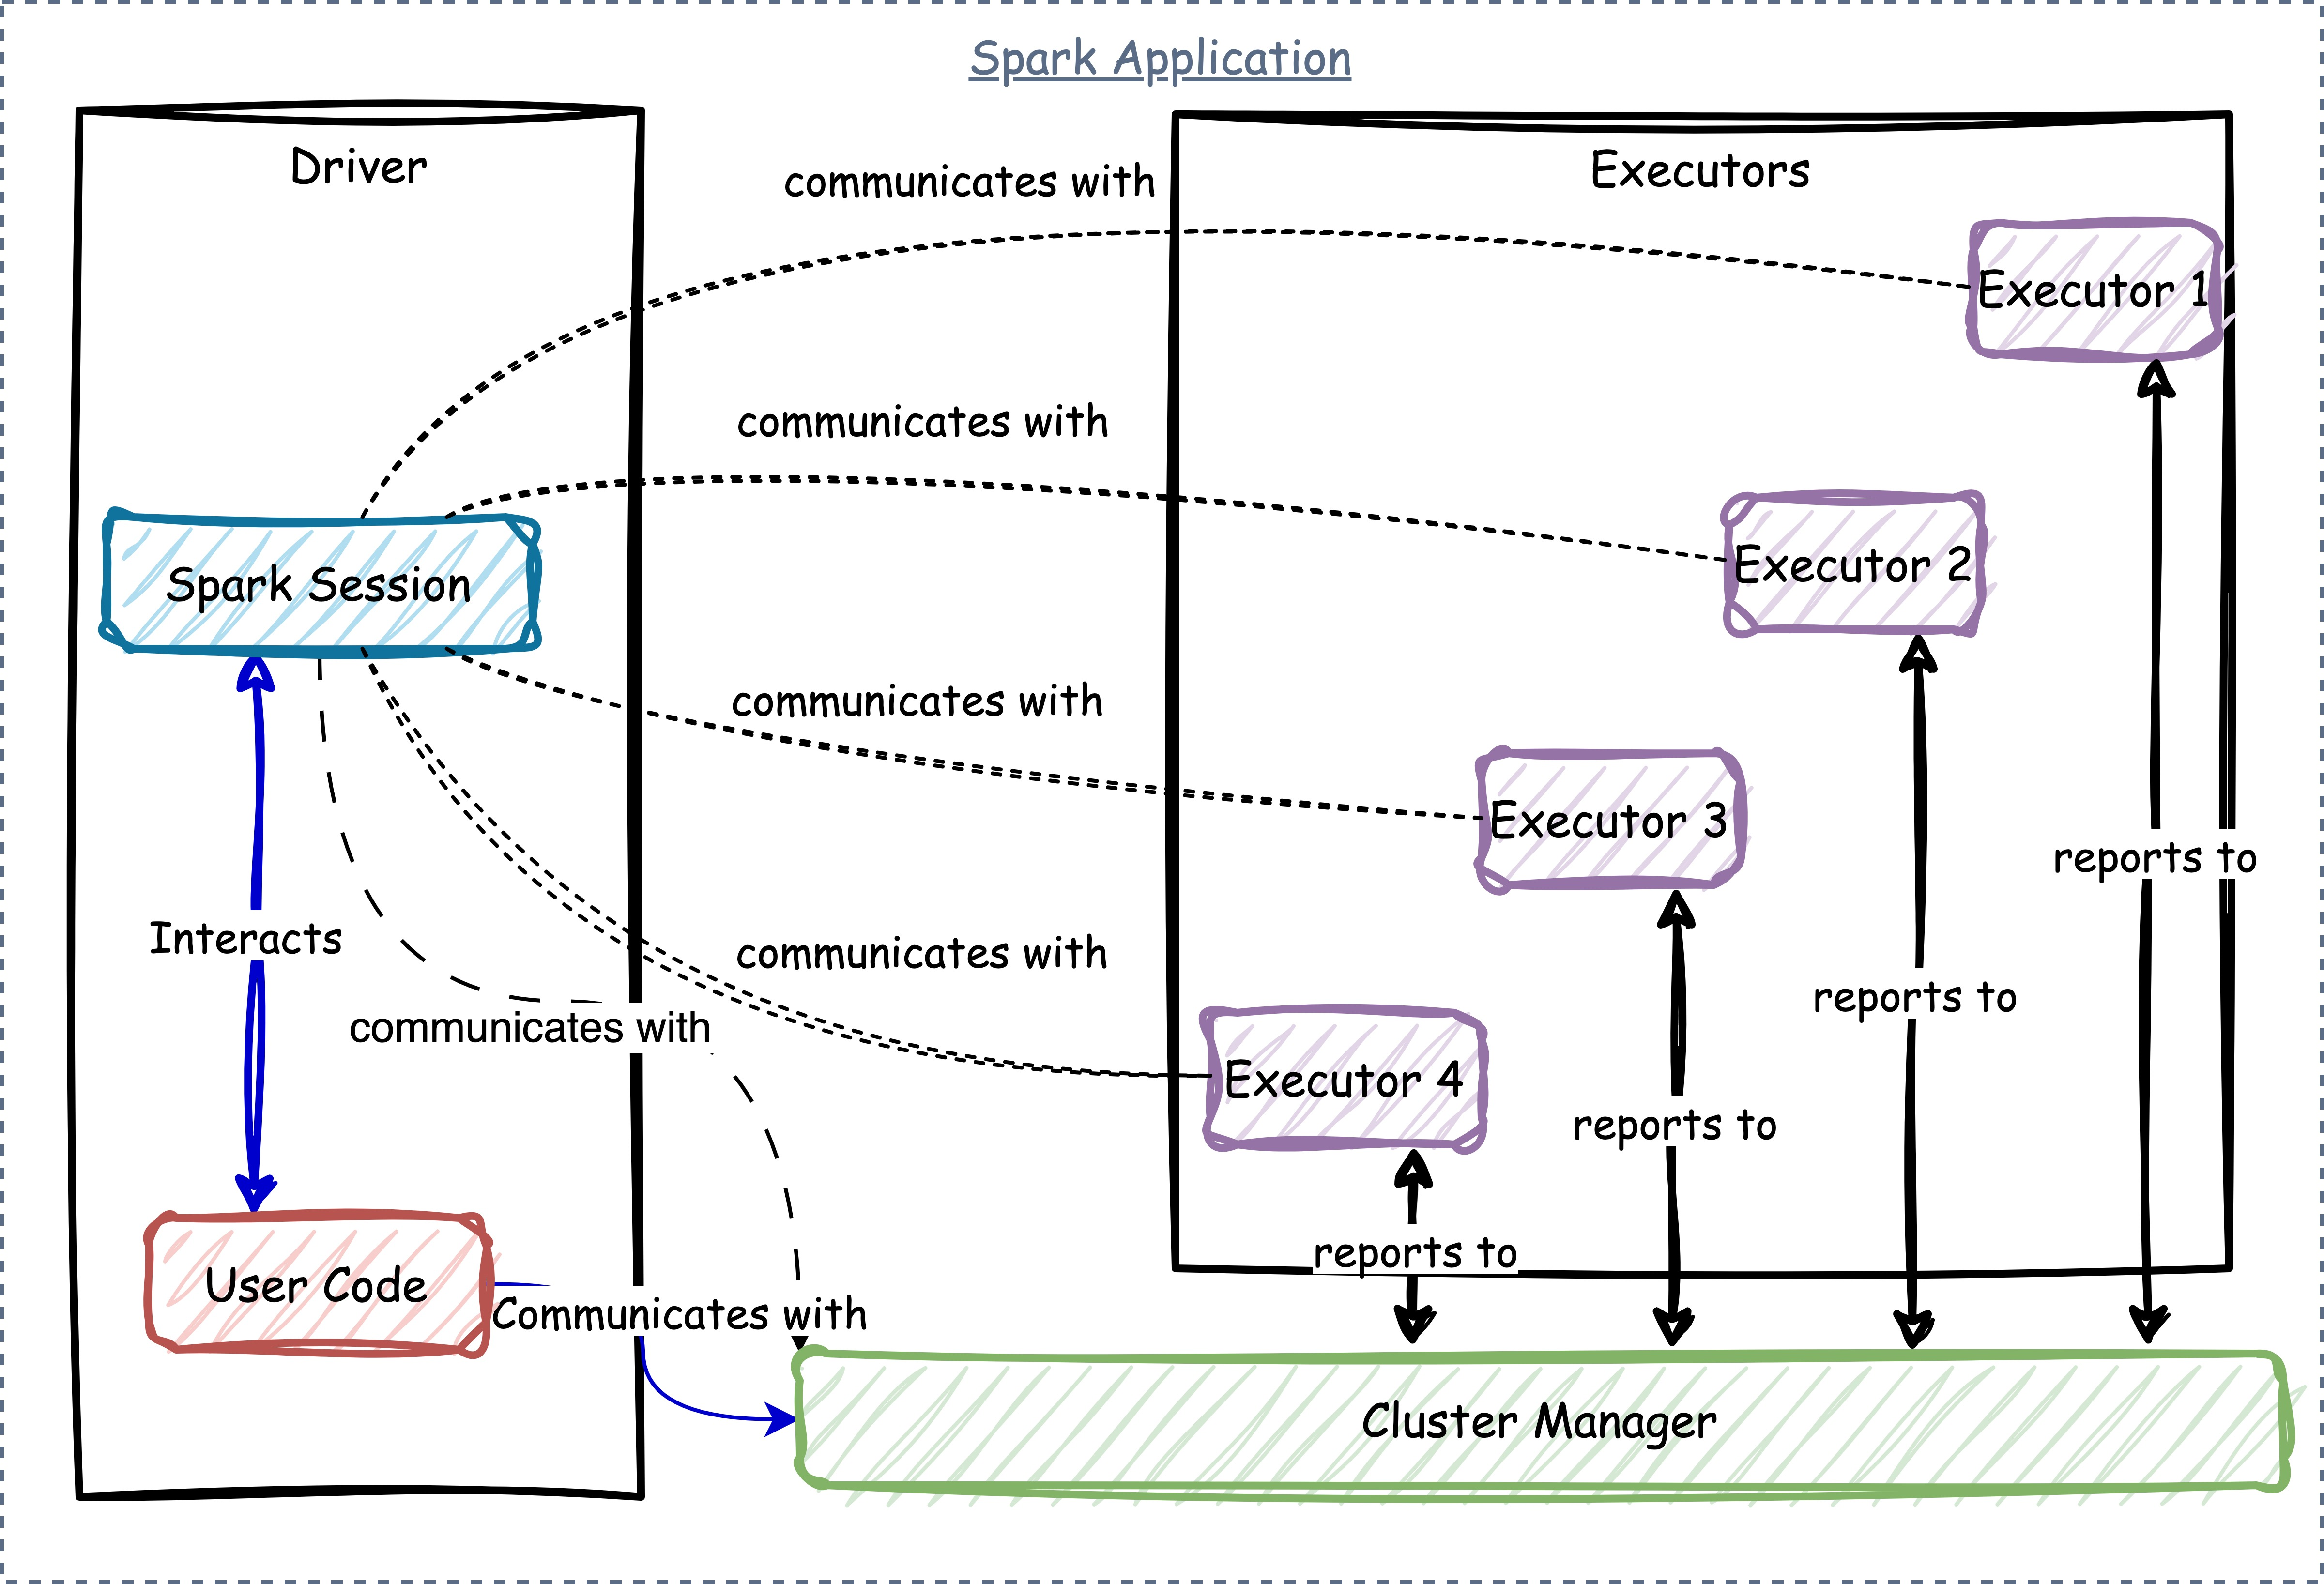
\includegraphics[width=\textwidth,height=.75\textheight,keepaspectratio]{./Figures/chapter-04/SparkCourse.drawio}\footnote{Spark the definitive guide, Ch.02}

\end{frame}

% Ch.04-14   | Spark Driver

\subsection{Spark Driver}\label{subsec:spark-driver}

\begin{frame}
    \frametitle{Spark Driver}
    The driver is the process \texttt{\color{blue}in the driver seat.}\footnote{Spark: The Definitive Guide, Chapter 15.} of your Spark Application.

\end{frame}

\begin{frame}
    \frametitle{Spark Driver: Key functions}


    \begin{itemize}
        \item It transforms all the Spark operations into DAG computations, schedules them, and distributes their execution as tasks across the Spark executors.
        \item Controlling the execution of a Spark Application.

    \end{itemize}

\end{frame}


\begin{frame}
    \frametitle{Spark Driver: Key functions}

    \begin{itemize}
        \item Acting as a process on a physical machine, responsible for the overall state of the application on the cluster.
        \item It instantiates the \texttt{\color{blue} SparkSession}
        \item It requests resources  (CPU, memory, etc.) from the cluster manager for Spark’s executors (JVMs).
        \item Once the resources are allocated, it communicates directly with the executors.
    \end{itemize}

\end{frame}


\begin{frame}
    \frametitle{Spark Driver: Recap}
%graph TD;
%    A[Spark Driver] -->|Schedules Tasks| B(DAG Scheduler);
%    A -->|Request Resources| C(Cluster Manager);
%    A -->|Communicates| D(Executors);
%    A -->|Initiates| E(SparkSession);
%    B -->|Distributes Tasks| D;
%    C -->|Grants Resources| D;
%    D -->|Executes Tasks| F(Task);
%    E -->|User Interface| G(Application Code);
%
    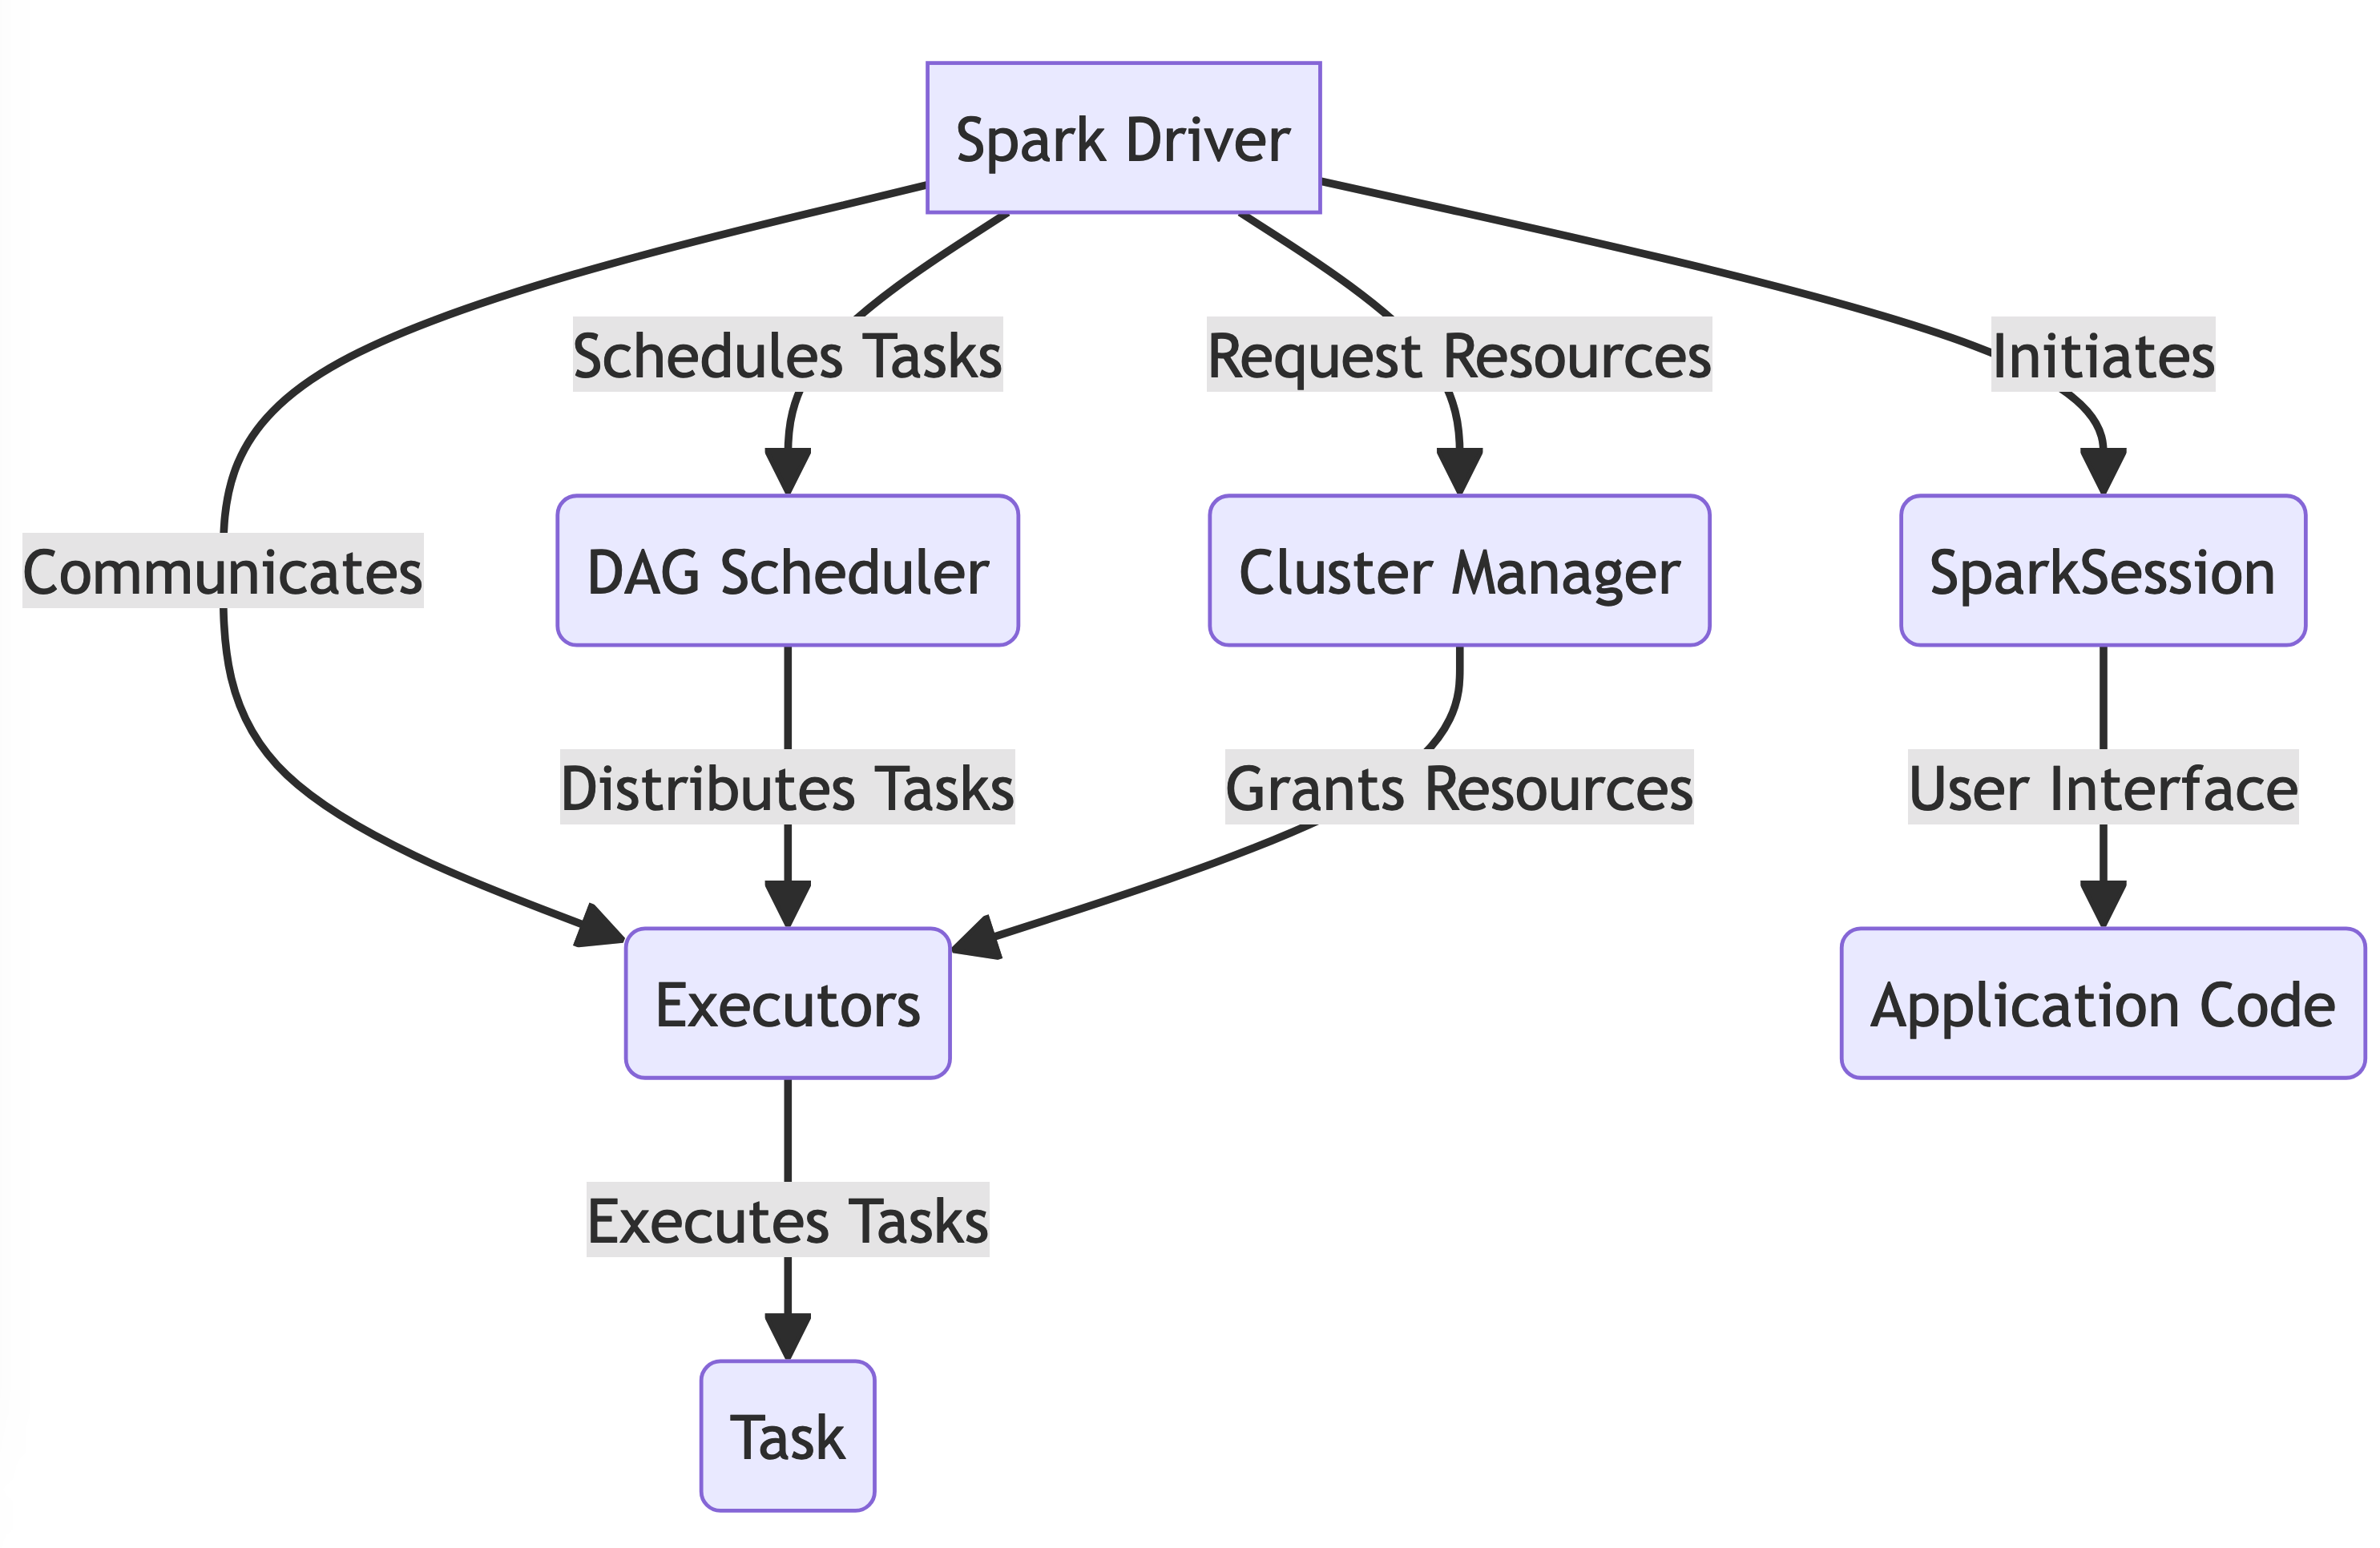
\includegraphics[width=\textwidth,height=.85\textheight,keepaspectratio]{./Figures/chapter-04/Mairmaid_SparkDriver}

\end{frame}

% Ch.04-15   | Spark Session

\subsection{Spark Distributed Execution: SparkSession}\label{subsec:spark-session}
\begin{frame}
    \frametitle{What is a Session?}

    \begin{itemize}
        \item A session refers to an interaction between two or more entities.
        \item In computing, it's especially common in networked computers on the internet.
    \end{itemize}

\end{frame}

\begin{frame}
    \frametitle{Types of Sessions in Computing}

    \begin{itemize}
        \item TCP session: A basic form of interaction in network communication.
        \item Login session: The period when a user is logged into a system.
        \item HTTP session: A series of interactions between a web server and a client.
        \item User session: The time a user interacts with a software application.
    \end{itemize}

\end{frame}

\begin{frame}
    \frametitle{Introducing SparkSession}

    \begin{itemize}
        \item Similar to the sessions mentioned, Spark has its own SparkSession.
        \item SparkSession provides a unified entry point to Spark's functionalities.
    \end{itemize}

\end{frame}

\begin{frame}
    \frametitle{Functionality of SparkSession}

    \begin{itemize}
        \item \textbf{SparkSession:} An object that provides a point of entry to interact with underlying Spark functionality.
        \item It allows programming Spark with its APIs.
        \item In an interactive Spark shell, the Spark driver instantiates a SparkSession for you.
        \item In a Spark application, you create a SparkSession object yourself.
        \item You can program Spark using DataFrame and Dataset APIs through SparkSession.
        \item In Scala and Python, the variable is available as \texttt{spark} when you start the console.

    \end{itemize}
\end{frame}

\begin{frame}
    \frametitle{SparkSession}
    \begin{itemize}
        \item The SparkSession instance is the way Spark executes user-defined manipulations across the cluster.
        \item There is a one-to-one correspondence between a SparkSession and a Spark Application.
        \item It connects the Spark driver program with the cluster manager.
        \item SparkSession determines the resource manager (YARN, Mesos, or Standalone) for communication.
        \item It allows configuration of Spark parameters.
    \end{itemize}
\end{frame}


\begin{frame}[fragile]
    \frametitle{Interacting with Spark in Earlier Versions}

    \begin{itemize}
        \item In earlier versions of Spark, setting up a Spark application required creating a SparkConf and SparkContext.
    \end{itemize}

    \begin{lstlisting}[language=Python,label={lst:pyspark-spark-context},caption={Create SparkContext in old Spark versions}]
from pyspark import SparkConf, SparkContext
from pyspark.sql import SQLContext

sparkConf = SparkConf().setAppName("SparkSessionExample").setMaster("local")
sc = SparkContext(conf=sparkConf)
sqlContext = SQLContext(sc)
    \end{lstlisting}

\end{frame}

%
\begin{frame}[fragile]
    \frametitle{Interacting with Spark in Earlier Versions}

    \begin{lstlisting}[language=Scala,label={lst:scala-spark-context},caption={Scala: Create SparkContext in old Spark versions}]
//set up the spark configuration and create contexts
val sparkConf = new SparkConf().setAppName("SparkSessionZipsExample").setMaster("local")
val sc = new SparkContext(sparkConf)
sc.set("spark.some.config.option", "some-value")
val sqlContext = new org.apache.spark.sql.SQLContext(sc)
    \end{lstlisting}

\end{frame}

%
%
\begin{frame}[fragile]
    \frametitle{Simplification in Spark 2.0 with SparkSession}

    \begin{itemize}
        \item Spark 2.0 introduced SparkSession, simplifying the way you interact with Spark.
        \item SparkSession encapsulates SparkConf, SparkContext, and SQLContext.
    \end{itemize}

    \begin{lstlisting}[language=Python,label={lst:spark-session-python-example},caption={Pyspark: Create SparkSession}]
from pyspark.sql import SparkSession

spark = SparkSession.builder \
    .appName("SparkSessionExample") \
    .config("spark.some.config.option", "value") \
    .getOrCreate()
    \end{lstlisting}
\end{frame}
%
\begin{frame}[fragile]
    \frametitle{Simplification in Spark 2.0 with SparkSession}
    \begin{lstlisting}[language=Scala,label={lst:spark-session-scala-example},caption={Spark: Create SparkSession}]
// Create a SparkSession. No need to create SparkContext.
val warehouseLocation = "file:${system:user.dir}/spark-warehouse"
val spark = SparkSession
   .builder()
   .appName("SparkSessionZipsExample")
   .config("spark.sql.warehouse.dir", warehouseLocation)
   .enableHiveSupport()
   .getOrCreate()
    \end{lstlisting}
\end{frame}

\begin{frame}
    \frametitle{Using SparkSession}
    \begin{itemize}
        \item Spark 2.0 introduces SparkSession.
        \item With SparkSession, you can access all Spark functionalities.
        \item A unified entry point to Spark's functionality, reduces the need for multiple context initializations.
        \item Encapsulates the functionalities of SQLContext, HiveContext, and more.
    \end{itemize}
\end{frame}

\begin{frame}
    \frametitle{Reference}
    \begin{itemize}
        \item The examples shown are based on a blog post from Databricks.
        \item URL: \url{https://www.databricks.com/blog/2016/08/15/how-to-use-sparksession-in-apache-spark-2-0.html}
    \end{itemize}
\end{frame}
%
%%Ch.04-16   | Spark Cluster Manager
%
%\subsection{Cluster manager}\label{subsec:cluster-manager}
%
%\begin{frame}
%    \frametitle{Introduction to Spark Cluster Managers}
%    \begin{itemize}
%        \item The cluster manager allocates resources for Spark applications.
%        \item Supports several managers: Standalone, Hadoop YARN, Apache Mesos, and Kubernetes.
%    \end{itemize}
%\end{frame}
%
%\begin{frame}
%    \frametitle{Role of the Cluster Manager}
%    \begin{itemize}
%        \item The Spark Driver and Executors do not exist in a void, and this is where the cluster manager
%        comes in.
%        \item The cluster manager is important for managing a cluster of machines intended to run Spark Applications.
%        \item Maintains a \texttt{driver (or master)} and \texttt{worker} nodes, tied to \textbf{physical machines}.
%    \end{itemize}
%\end{frame}
%
%
%\begin{frame}
%    \frametitle{Cluster Manager Components}
%    \begin{figure}
%        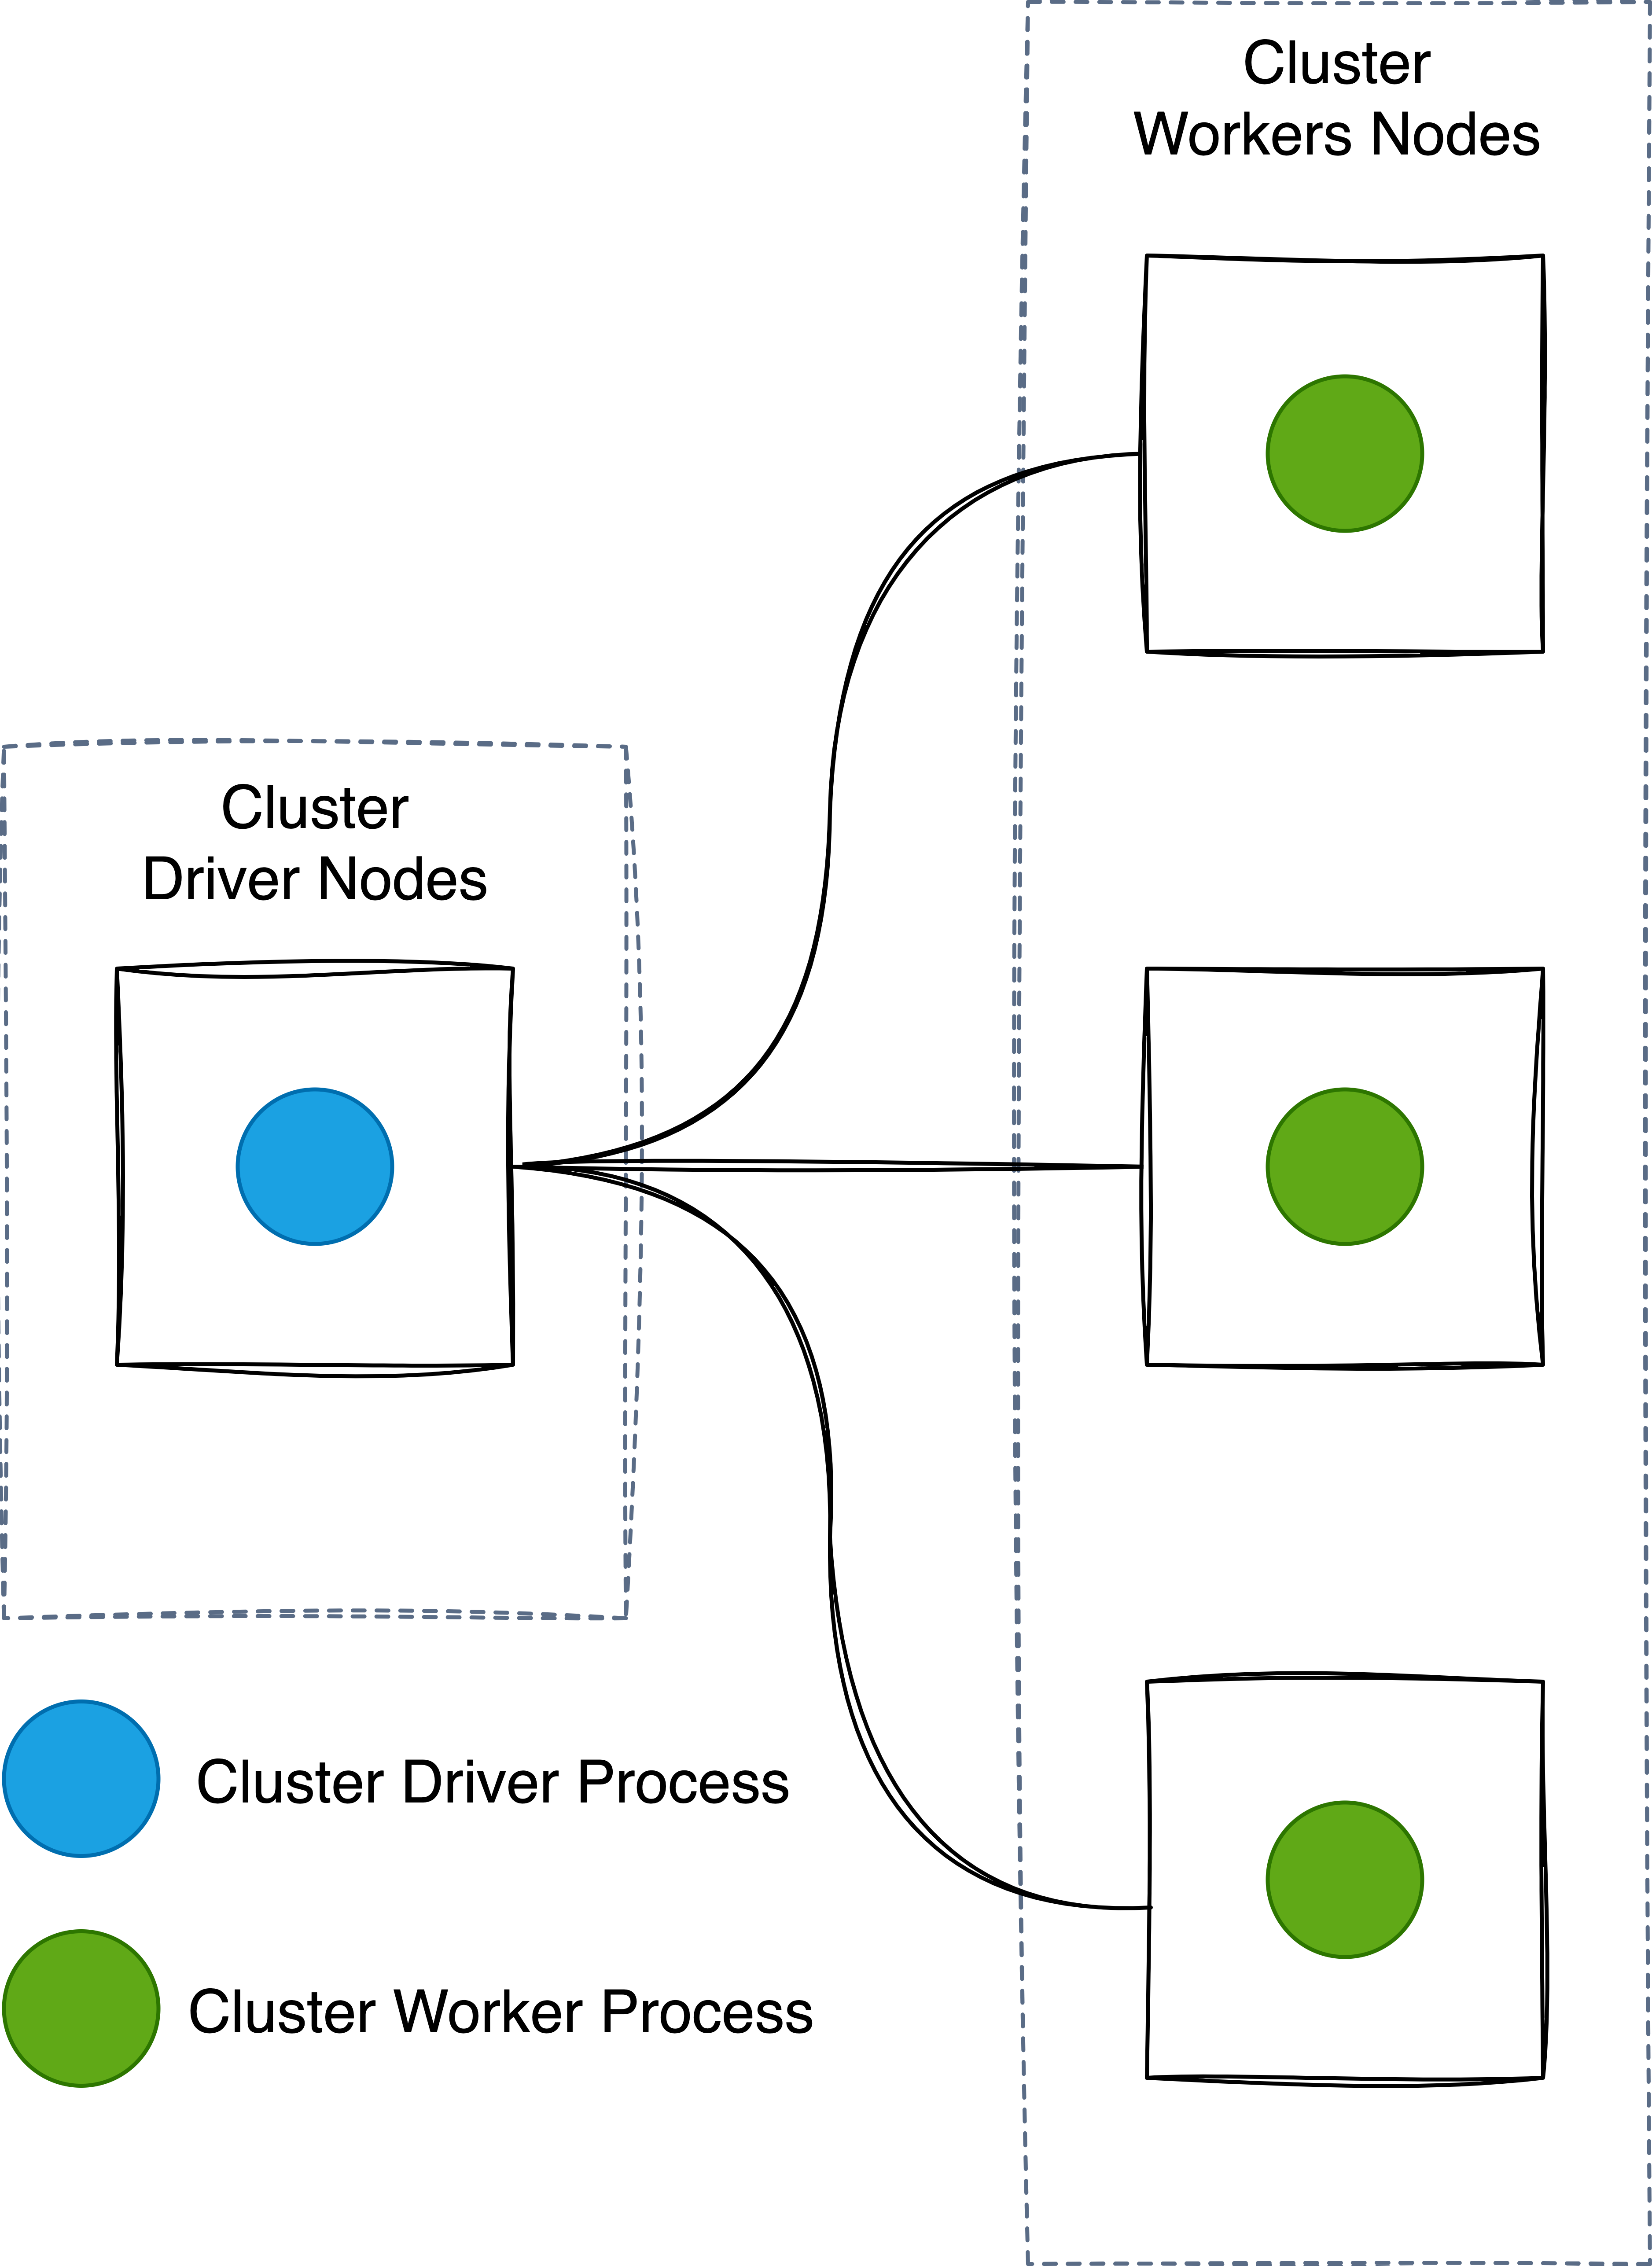
\includegraphics[width=\textwidth,height=.7\textheight,keepaspectratio]{./Figures/chapter-04/cluster_manager_processes}
%        \caption{A cluster driver and worker (no Spark Application yet).}\label{fig:cluster_manager_processes}
%    \end{figure}
%\end{frame}
%
%\begin{frame}
%    \frametitle{Execution of Spark Applications}
%    \begin{itemize}
%        \item The user requests resources from the cluster manager to initiate Spark applications.
%        \item The user configures the application to specify resources for the driver or only for executors.
%        \item The cluster manager directly manages the machines during the execution of the application.
%    \end{itemize}
%\end{frame}
%
%% Ch.04-17   | Spark Execution Mode
%
%\subsection{Execution Modes}\label{subsec:deployment-mode}
%\begin{frame}
%    \frametitle{Execution Modes Overview}
%    \begin{itemize}
%        \item Execution modes define the location of resources when running Spark applications.
%        \item Three modes available:
%        \begin{enumerate}
%            \item Cluster mode
%            \item Client mode
%            \item Local mode
%        \end{enumerate}
%    \end{itemize}
%\end{frame}
%
%\begin{frame}
%    \frametitle{Cluster Manager Components}
%    \begin{figure}
%        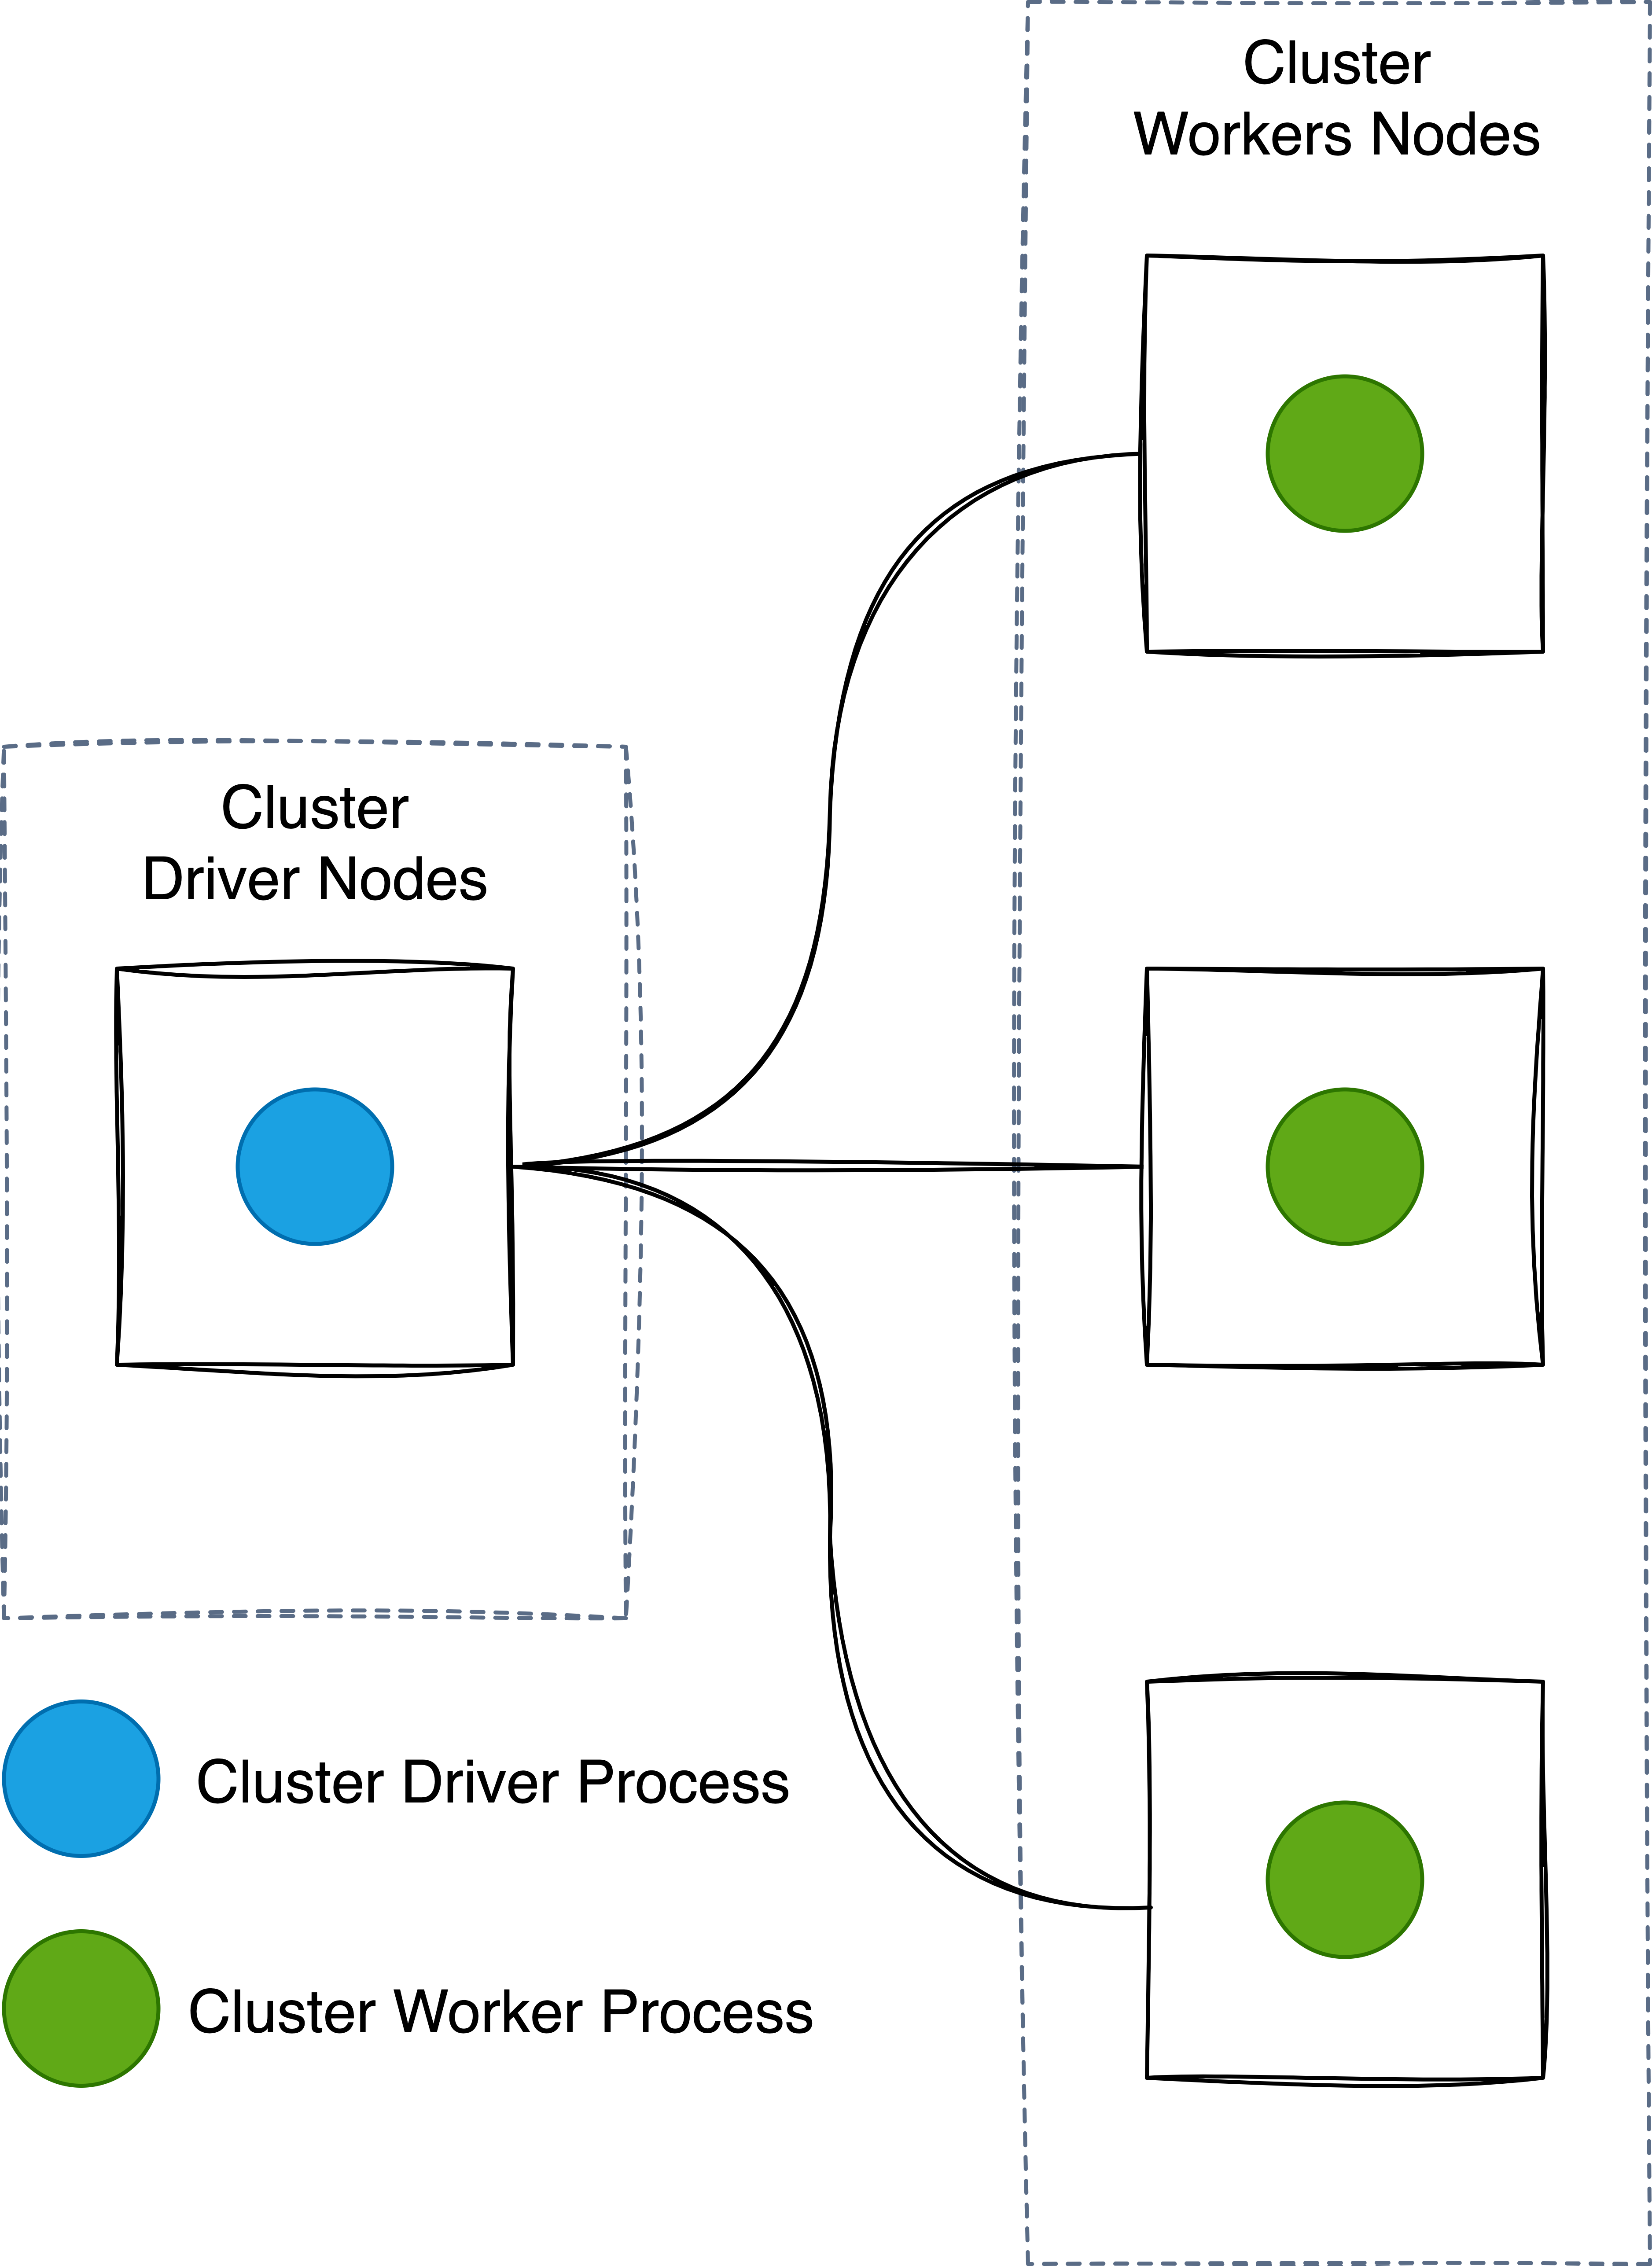
\includegraphics[width=\textwidth,height=.7\textheight,keepaspectratio]{./Figures/chapter-04/cluster_manager_processes}
%        \caption{A cluster driver and worker (no Spark Application yet).}\label{fig:cluster-manager-components}
%    \end{figure}
%\end{frame}
%
%\begin{frame}
%    \frametitle{Cluster Mode}
%    \begin{itemize}
%        \item Most common mode for running Spark Applications.
%        \item User submits a pre-compiled JAR, Python script, or R script to a cluster manager.
%        \item The cluster manager then launches the driver process on a worker node inside the cluster.
%        \item Executor processes also launched within the cluster.
%        \item Cluster manager handles all Spark Application processes.
%        \item This means that the cluster manager is responsible for maintaining all Spark Application–related processes.
%    \end{itemize}
%\end{frame}
%
\begin{frame}
    \frametitle{Spark Cluster Mode}
    \begin{figure}
        \includegraphics[width=\textwidth,height=.7\textheight,keepaspectratio]{./Figures/chapter-04/spark_cluster_mode}
        \caption{Spark’s cluster mode.}\label{fig:cluster_mode}
    \end{figure}
\end{frame}
%
\begin{frame}
    \frametitle{Client Mode}
    \begin{itemize}
        \item Similar to cluster mode, but the \textbf{\texttt{Spark driver remains on the client
        machine that submitted the application}}.
        \item \textbf{Client machine} is responsible for maintaining the Spark driver process.
        \item \textbf{Cluster manager} maintains executor processes.
        \item Commonly used with gateway machines or edge nodes.
        \item The driver is running on a machine outside of the cluster but that the workers are located on machines in the cluster.
    \end{itemize}
\end{frame}
%
\begin{frame}
    \frametitle{Spark Client Mode}
    \begin{figure}
        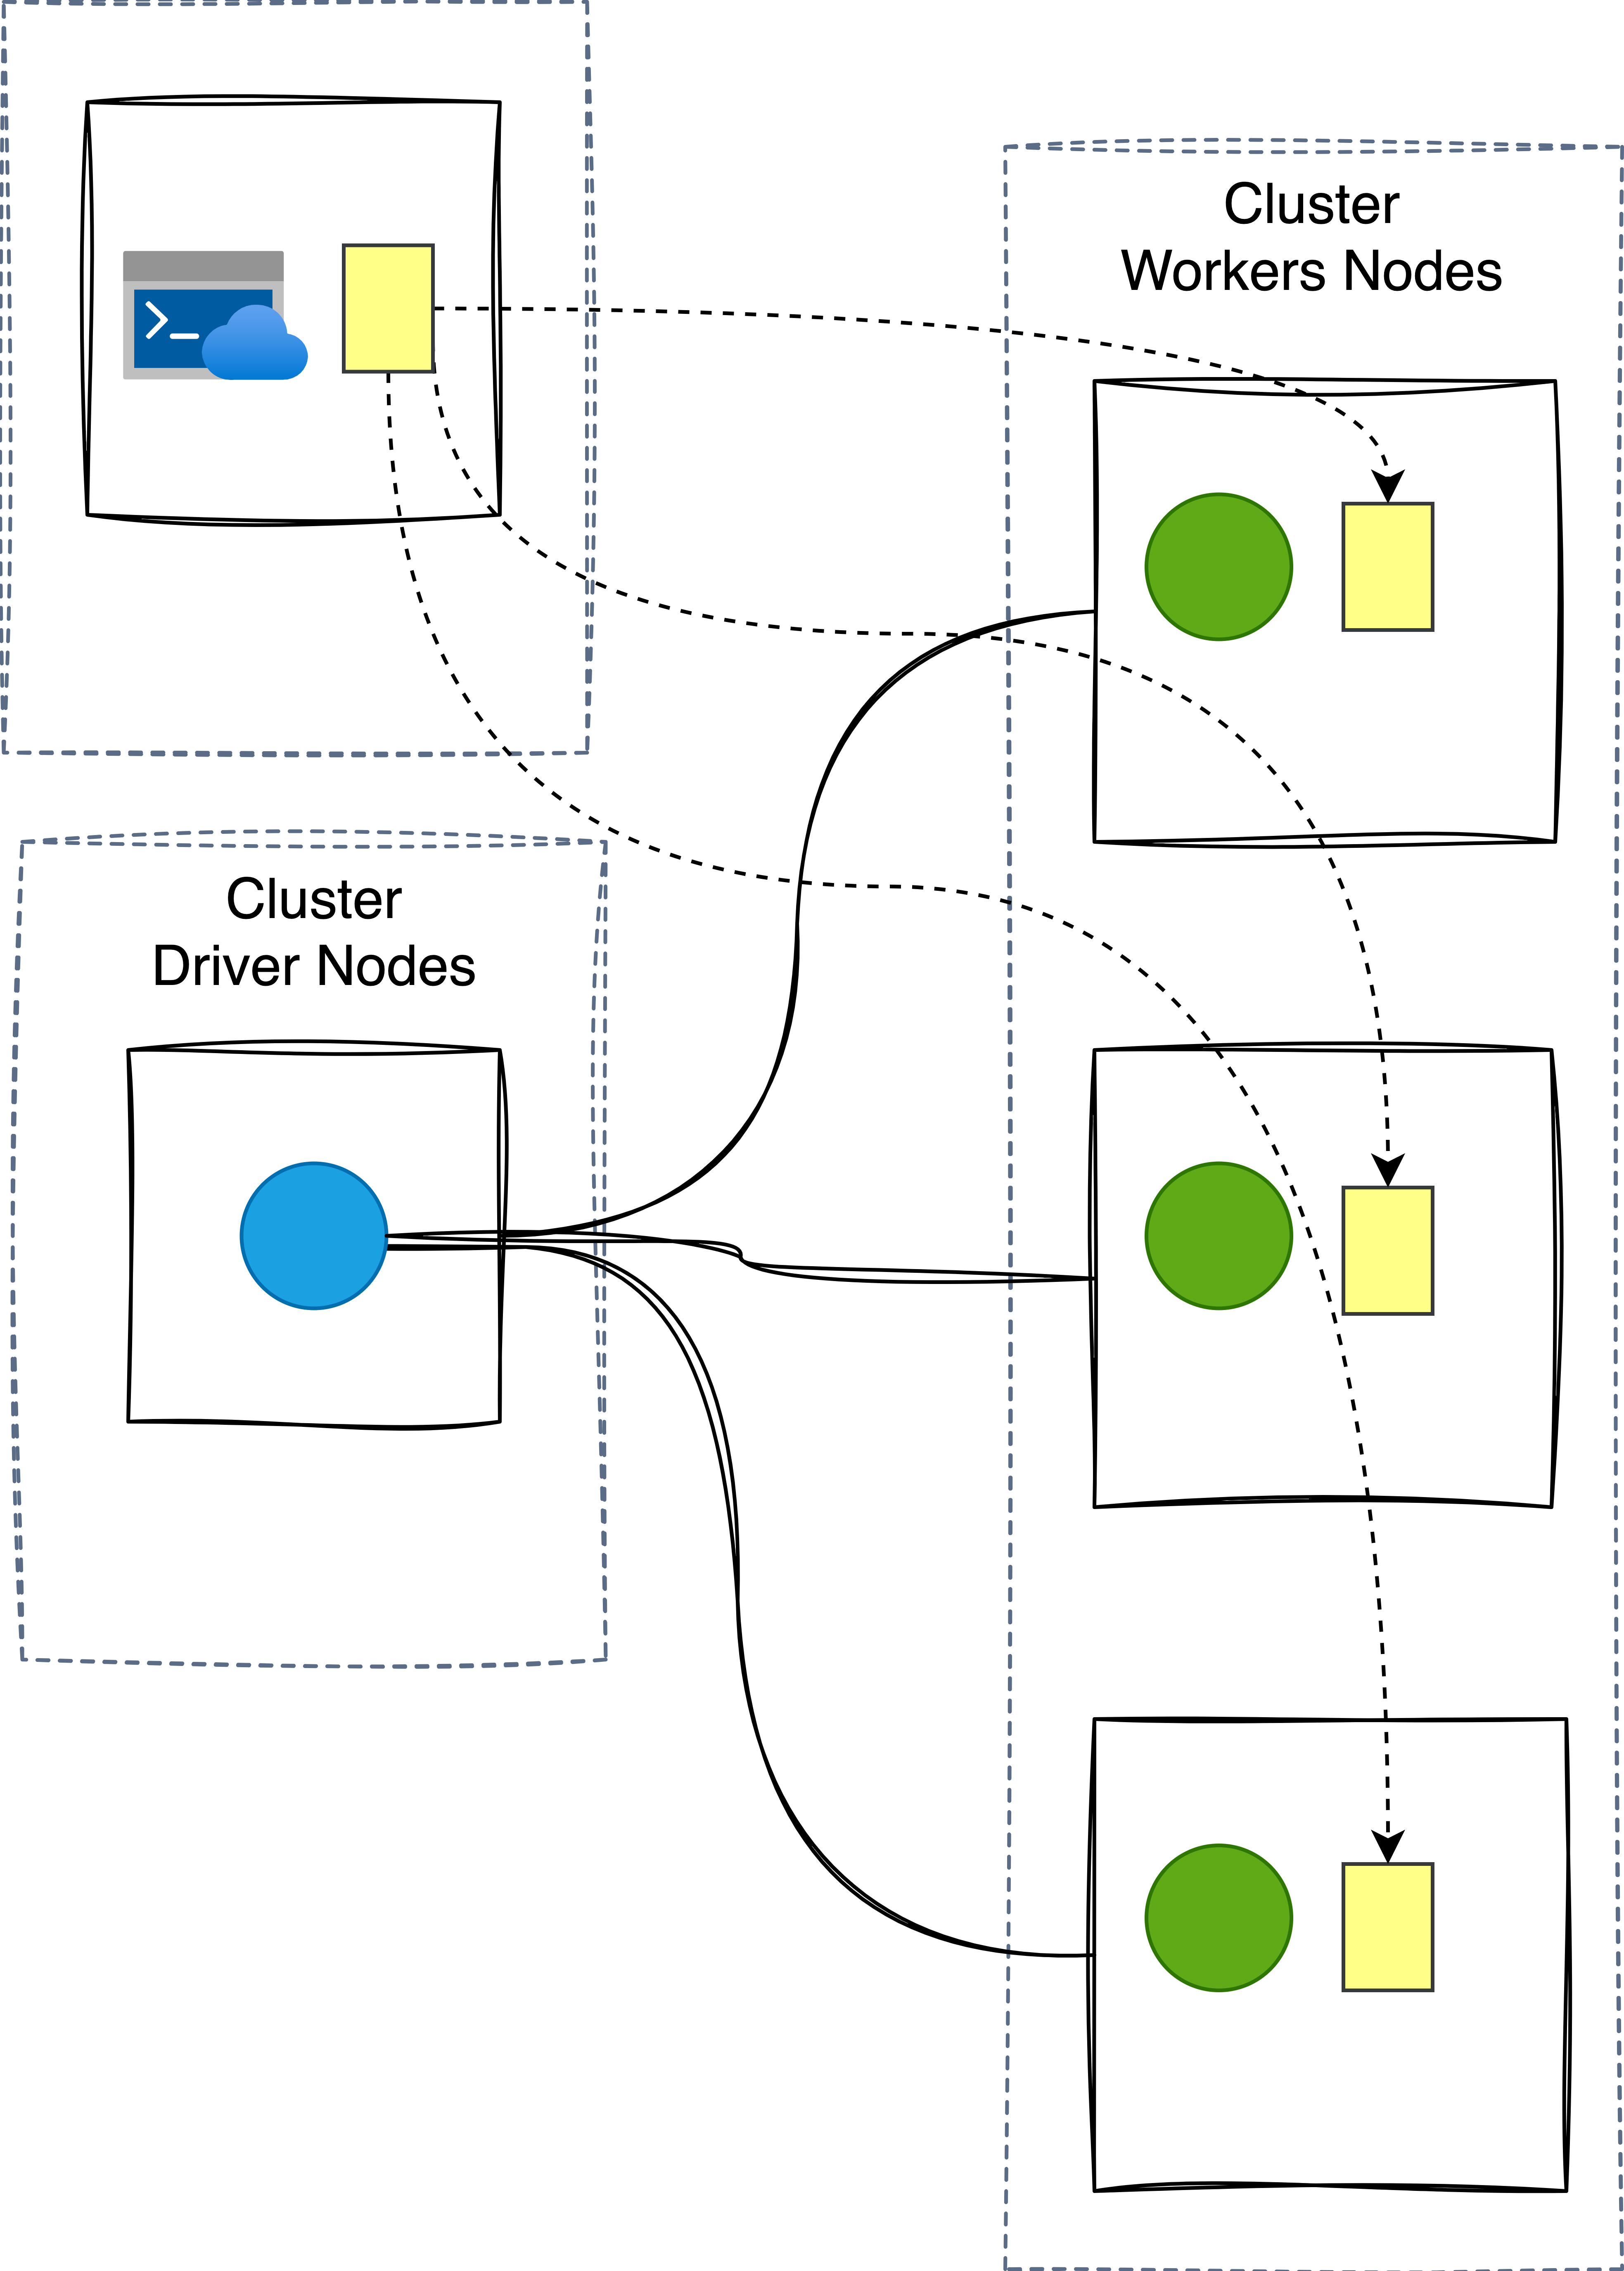
\includegraphics[width=\textwidth,height=.7\textheight,keepaspectratio]{./Figures/chapter-04/spark_client_mode}
        \caption{Spark’s client mode.}\label{fig:client_mode}
    \end{figure}
\end{frame}
%
\begin{frame}
    \frametitle{Local Mode}
    \begin{itemize}
        \item Runs the entire application on a single machine.
        \item Parallelism achieved through threads on the same machine.
        \item Ideal for learning, testing, or local development.
        \item Not recommended for production use.
    \end{itemize}
\end{frame}
%
%%\begin{frame}
%%    \frametitle{Spark Deployment Modes Cheat Sheet}
%%    \begin{table}[h!]
%%        \centering
%%        \resizebox{\textwidth}{!}{%
%%        \begin{tabular}{|p{2cm} |p{5cm} |p{5cm} |p{5cm}|}
%%            \hline
%%            \rowcolor{Gray}
%%            \textbf{Mode} & \textbf{Driver} & \textbf{Executor} & \textbf{Cluster Manager} \\
%%            \hline
%%            \textbf{Local} & Runs on a single JVM & Runs with driver & Single host \\
%%            \hline
%%            \textbf{Standalone} & Any cluster node & Own JVM per node & Any host in cluster \\
%%            \hline
%%            \textbf{YARN (client)} & Client machine & NodeManager container & YARN Resource Manager \\
%%            \hline
%%            \textbf{YARN (cluster)} & YARN App Master & Similar to client & Similar to client \\
%%            \hline
%%            \textbf{Kubernetes} & Kubernetes pod & Individual pods & Kubernetes Master \\
%%            \hline
%%        \end{tabular}
%%        }
%%        \caption{Summary of Spark deployment modes}\label{tab:spark-deployment}
%%    \end{table}
%%\end{frame}
%% Ch.04-18   | Spark Executors

\subsection{Spark executors}\label{subsec:spark-executors}

\begin{frame}
    \frametitle{Spark Executors}
    \begin{itemize}
        \item Executors are processes that run the tasks assigned by the driver.
        \item Each Spark Application has distinct executor processes.
        \item Typically, one executor runs per node in most deployment modes.
        \item Executors' main function: Execute tasks, return status, and communicate outcomes.
    \end{itemize}
\end{frame}

% Ch.04-19   | Spark Data Partitioning

\subsection{Data partition}\label{subsec:data-partition}


% Slide 1
\begin{frame}{Introduction to Data Distribution and Partitions}
    \begin{itemize}
        \item \textbf{Data Distribution:} Physical data is distributed across storage as partitions residing in either HDFS or cloud storage.
        \item \textbf{Data Abstraction:} Spark treats each partition as a high-level logical data abstraction—as a DataFrame in memory.
    \end{itemize}
\end{frame}

% Slide 2
\begin{frame}{Data Locality and Task Allocation}
    \begin{itemize}
        \item \textbf{Data Locality:} Each Spark executor is preferably allocated a task that requires it to read the partition closest to it in the network, observing data locality.
        \item \textbf{Optimal Task Allocation:} Partitioning allows for efficient parallelism.
        \item \textbf{Minimize Network Bandwidth:} A distributed scheme of breaking up data into chunks or partitions allows Spark executors to process only data that is close to them, minimizing network bandwidth.
    \end{itemize}
\end{frame}

% Slide 3
\begin{frame}{Benefits of Partitioning}
    \begin{itemize}
        \item \textbf{Efficient Parallelism:} Partitioning allows executors to process data close to them.
        \item \textbf{Dedicated Processing:} Each core on an executor works on its own partition, minimizing network bandwidth usage.
    \end{itemize}
\end{frame}

% Slide 4
\begin{frame}[fragile]{Practical Example - Distributing Data}
    \begin{lstlisting}[language=Python,label={lst:pyspark-data-partitioning}]
        log_df = spark.read.text("path_to_large_text_file").repartition(8)
        print(log_df.rdd.getNumPartitions())
    \end{lstlisting}
    This example splits data across clusters into eight partitions.
\end{frame}

% Slide 5
\begin{frame}[fragile]{Practical Example - Creating a DataFrame}
    \begin{lstlisting}[language=Python,label={lst:pyspark-creating-dataframe}]
        df = spark.range(0, 10000, 1, 8)
        print(df.rdd.getNumPartitions())
    \end{lstlisting}
    This creates a DataFrame of 10,000 integers over eight partitions in memory.
\end{frame}

% Slide 6
\begin{frame}{Conclusion}
    \begin{itemize}
        \item \textbf{Key Takeaway:} Efficient data partitioning is crucial for optimizing processing in Spark.
    \end{itemize}
\end{frame}

%%% Local Variables:
%%% mode: latex
%%% TeX-master: "../main"
% !TeX root = ../main.tex
%%% TeX-engine: xetex
%%% End: